\begin{frame}{Opis naloge}
  \begin{tikzpicture}[remember picture,overlay]
      \node[xshift=-2.7cm,yshift=3.6cm] at (current page.south east) {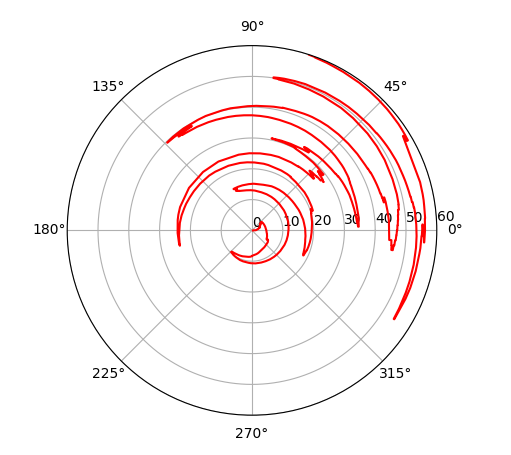
\includegraphics[width=6.0cm]{img/trace.png}};
  \end{tikzpicture}
  \vspace{-60pt}
  \begin{itemize}
    \item $360\degree$ video
    \item Učni podatki: 86 sledi pogledov uporabnikov
    \item Testni podatki
    \begin{itemize}
      \item $4s$ znanih kotov
      \item $4s$ neznanih kotov
    \end{itemize}
    \item Katere tokove naložiti v \\ predpomnilnik uporabnika?
  \end{itemize}
\end{frame}

\begin{frame}{Smiselna delitev naloge}
  \begin{itemize}
    \item Določanje kotov pogleda uporabnikov za $4$ neznane sekunde
    \item Določanje tokov ki jih pošljemo uporabniku
  \end{itemize}
\end{frame}

\begin{frame}{Analiza podatkov: vročinska slika}
  \begin{figure}
    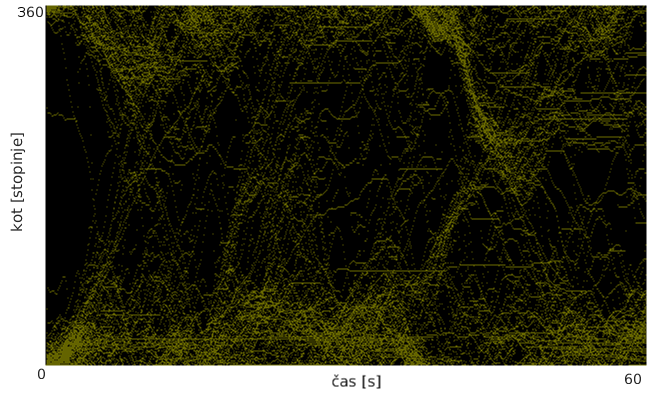
\includegraphics[scale=0.67]{img/hm-kd.png}
  \end{figure}
\end{frame}

\begin{frame}{Pomembnosti stolpcev v zornem kotu}
  \begin{tikzpicture}[remember picture,overlay]
      \node[xshift=6.3cm,yshift=0cm] at (current page.west) {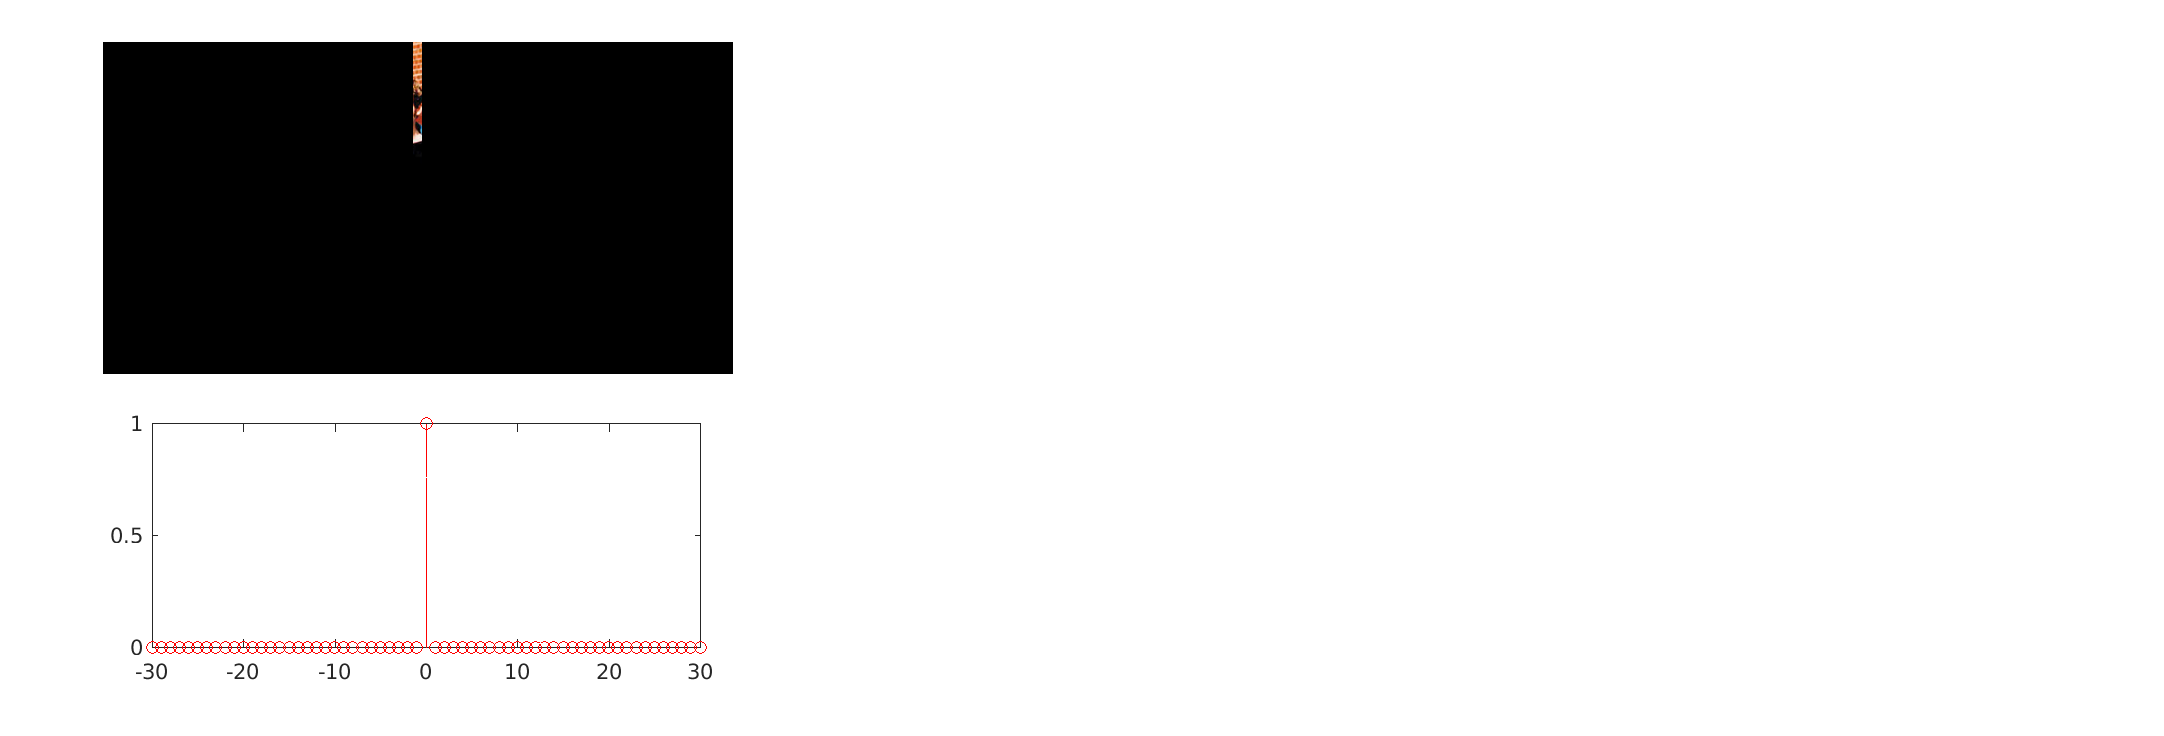
\includegraphics[width=12.0cm]{img/views1.png}};
  \end{tikzpicture}
\end{frame}

\begin{frame}{Pomembnosti stolpcev v zornem kotu}
  \begin{tikzpicture}[remember picture,overlay]
      \node[xshift=6.3cm,yshift=0cm] at (current page.west) {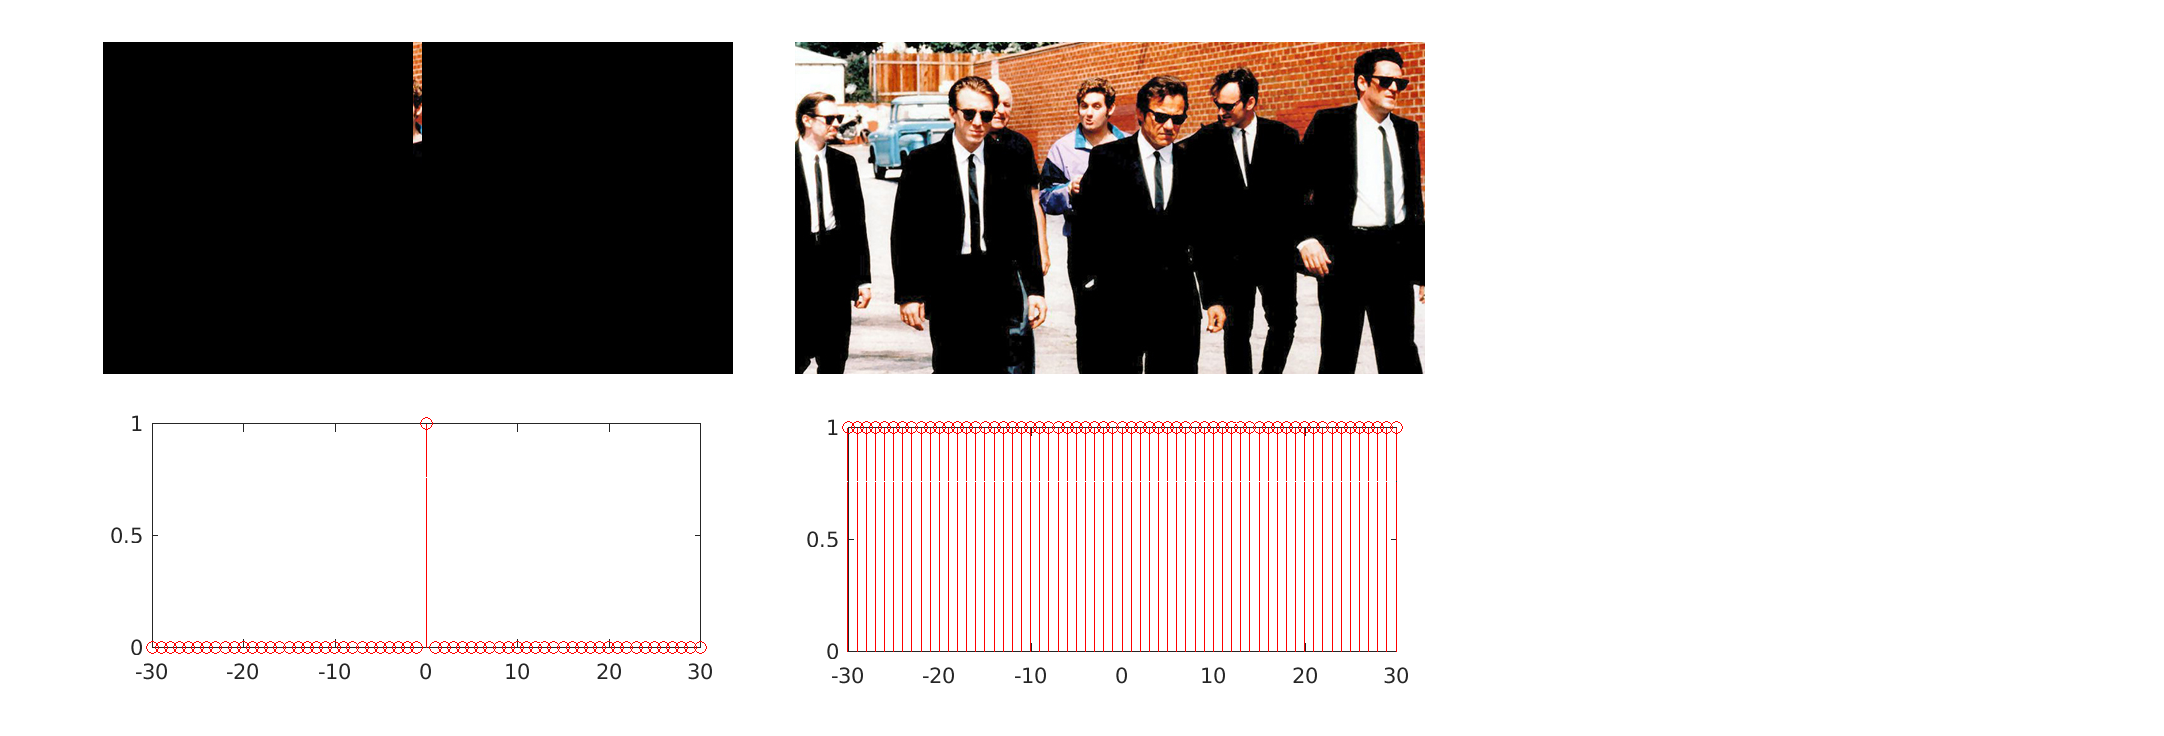
\includegraphics[width=12.0cm]{img/views2.png}};
  \end{tikzpicture}
\end{frame}

\begin{frame}{Pomembnosti stolpcev v zornem kotu}
  \begin{tikzpicture}[remember picture,overlay]
      \node[xshift=6.3cm,yshift=0cm] at (current page.west) {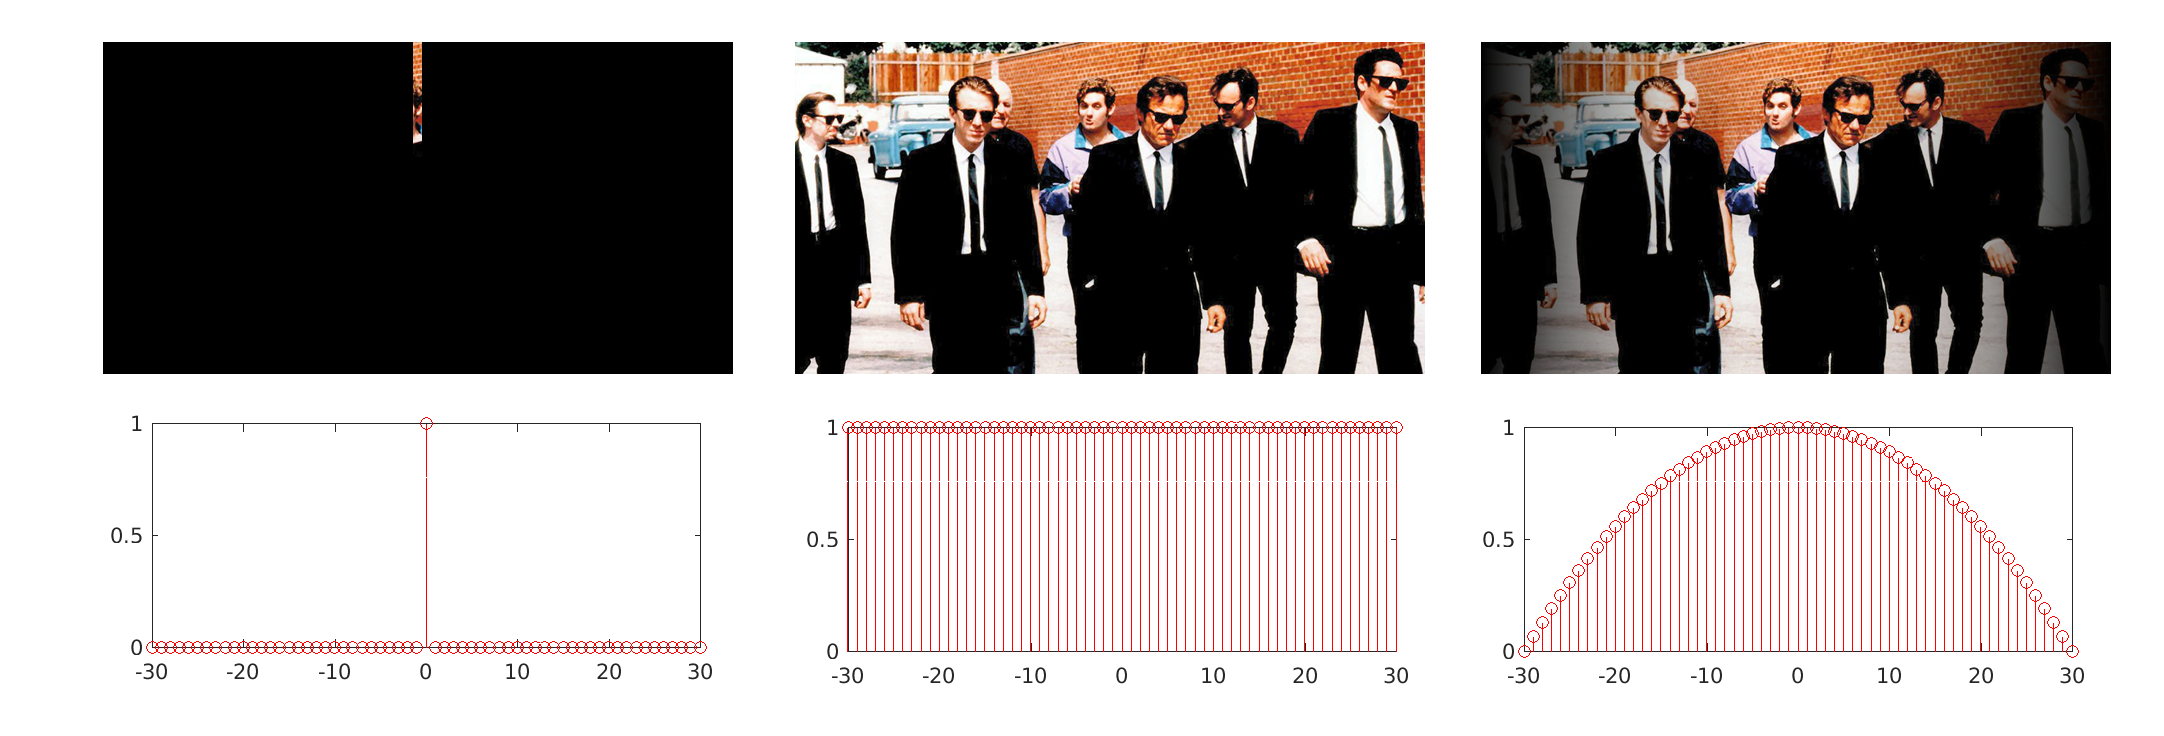
\includegraphics[width=12.0cm]{img/views3.png}};
  \end{tikzpicture}
\end{frame}

\begin{frame}{Vročinska slika z Welch oknom}
  \begin{figure}
    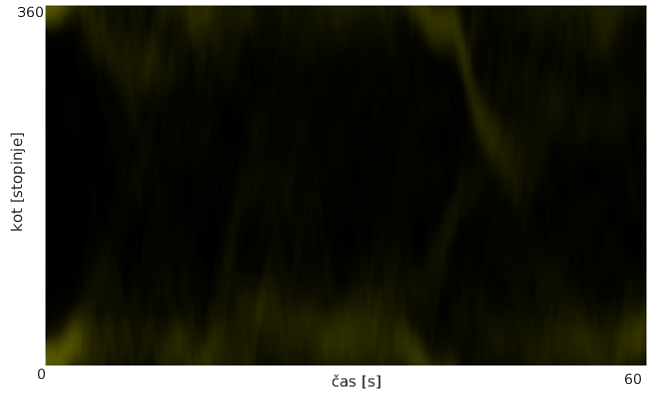
\includegraphics[scale=0.67]{img/hm-we.png}
  \end{figure}
\end{frame}

\begin{frame}{Vročinska slika z Welch oknom}
  \begin{figure}
    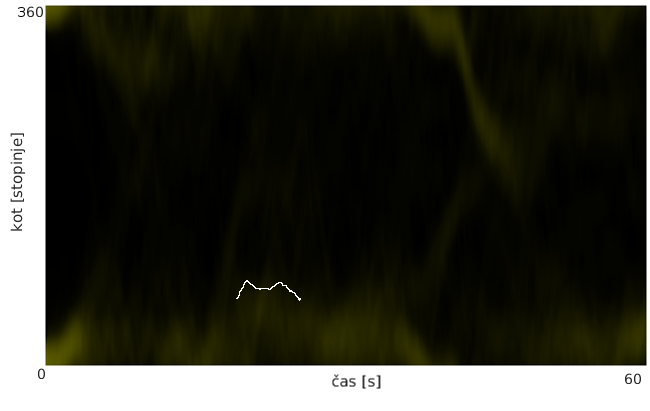
\includegraphics[scale=0.67]{img/hm-wet.png}
  \end{figure}
\end{frame}

\begin{frame}{Maksimiziranje rumene barve}
  \begin{itemize}
    \item Z uporabo dinamičnega programiranja
  \end{itemize}

\begin{displaymath}
  sc(\theta, t) = heatmap(\theta, t) + \left\{ \begin{array}{ll}
                                            0 & \textrm{če $t = 60$,}\\
                                            \displaystyle \max_{\theta'}\{w(\theta'-\theta) \cdot sc(\theta', t+1)\} & \textrm{sicer.}
  \end{array} \right.
\end{displaymath}
  \begin{figure}
    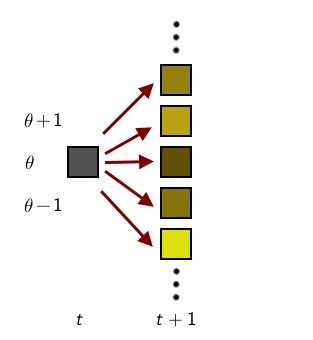
\includegraphics[scale=0.57]{img/dp.png}
  \end{figure}
\end{frame}

\begin{frame}{Maksimiziranje rumene barve}
  \begin{itemize}
    \item Z uporabo dinamičnega programiranja
  \end{itemize}

\begin{displaymath}
  sc(\theta, t) = heatmap(\theta, t) + \left\{ \begin{array}{ll}
                                            0 & \textrm{če $t = 60$,}\\
                                            \displaystyle \max_{\theta'}\{w(\theta'-\theta) \cdot sc(\theta', t+1)\} & \textrm{sicer.}
  \end{array} \right.
\end{displaymath}
  \begin{figure}
    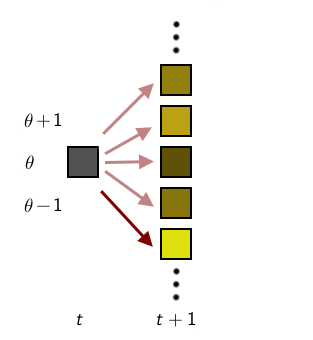
\includegraphics[scale=0.57]{img/dp2.png}
  \end{figure}
\end{frame}

\begin{frame}{Analiza podatkov: relativni premiki uporabnikov}
  \begin{figure}
    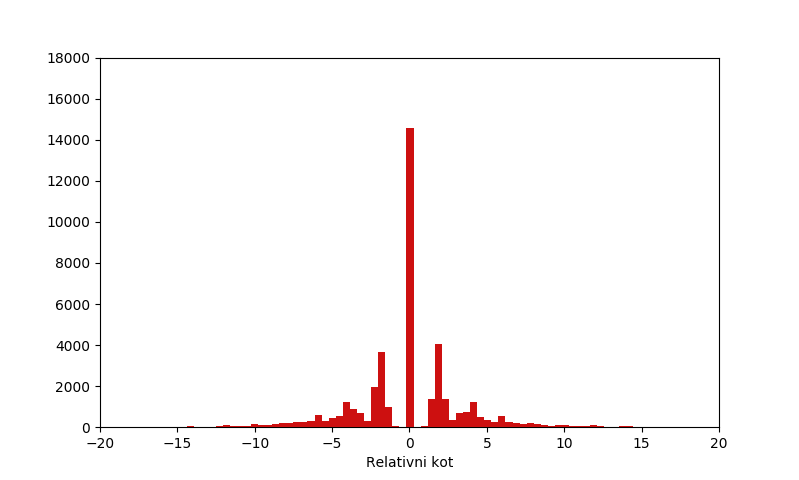
\includegraphics[scale=0.55]{img/rel_moves.png}
  \end{figure}
\end{frame}

\begin{frame}{Maksimiziranje rumene barve}
  \begin{itemize}
    \item Z uporabo dinamičnega programiranja
  \end{itemize}

\begin{displaymath}
  sc(\theta, t) = heatmap(\theta, t) + \left\{ \begin{array}{ll}
                                            0 & \textrm{če $t = 60$,}\\
                                            \displaystyle \max_{\theta'}\{w(\theta'-\theta) \cdot sc(\theta', t+1)\} & \textrm{sicer.}
  \end{array} \right.
\end{displaymath}
  \begin{figure}
    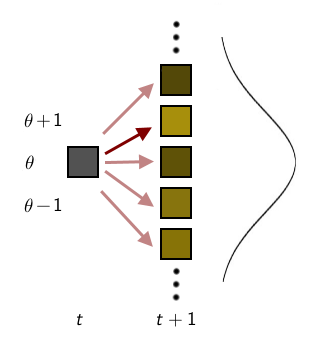
\includegraphics[scale=0.57]{img/dp3.png}
  \end{figure}
\end{frame}

\begin{frame}{Razbitje videa na tokove}
  \begin{itemize}
    \item Izhodišče: želimo zagotoviti optimalno kvaliteto za znane 4 sekunde
  \end{itemize}
\end{frame}

\begin{frame}{Razbitje videa na tokove}
  \begin{itemize}
    \item 90 tokov po $4\degree$ kvalitete $100\%$
    \item 1 tok $360\degree$ kvalitete $1\%$
    \item Želimo čim pokriti čim več kotov na vsako stran
  \end{itemize}
  \begin{figure}
    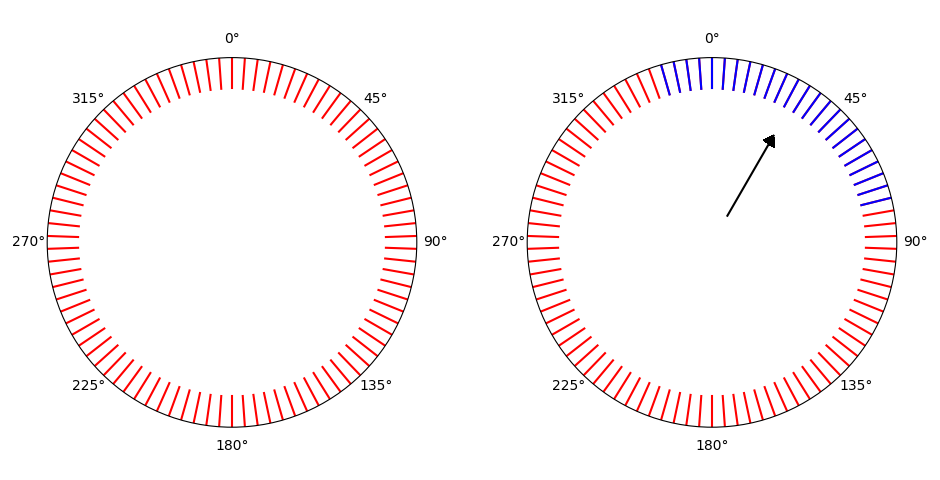
\includegraphics[scale=0.4]{img/streams.png}
  \end{figure}
\end{frame}

\begin{frame}{Nastavljanje parametrov}
  \begin{itemize}
    \item Parametri:
    \begin{itemize}
      \item Resolucija vročinske slike
      \item Okno pri vročinski sliki
      \item Uteži pri DP
      \item Različne strategije za tokove
    \end{itemize}
    \item Nastavimo s pomočjo prečnega preverjanja
  \end{itemize}
\end{frame}

\begin{frame}{Problemi}
  \begin{itemize}
    \item DP ne da nujno optimalne poti
    \item Če uporabniku preveč napačno napovemo kot, bo gledal kvaliteto $1\%$
    \item \ldots
  \end{itemize}
\end{frame}

\begin{frame}{}
  \centering
  \huge{Vprašanja?}
\end{frame}
